\documentclass[11pt]{article}

\usepackage[margin=1.05in]{geometry}
\usepackage{amsmath,amssymb,amsthm}
\usepackage{stmaryrd}
\usepackage{booktabs}
\usepackage{enumitem}
\usepackage{tikz}
\usepackage{listings}
\usepackage[T1]{fontenc}
\usepackage[expansion=false]{microtype}
\usepackage{hyperref}
\usetikzlibrary{arrows.meta,positioning,decorations.pathmorphing,calc}

\hypersetup{colorlinks=true, linkcolor=blue!45!black,
            citecolor=blue!45!black, urlcolor=blue!45!black}

\theoremstyle{plain}
\newtheorem{theorem}{Theorem}[section]
\newtheorem{proposition}[theorem]{Proposition}
\newtheorem{lemma}[theorem]{Lemma}
\newtheorem{corollary}[theorem]{Corollary}
\newtheorem{conjecture}[theorem]{Conjecture}
\theoremstyle{definition}
\newtheorem{definition}[theorem]{Definition}
\newtheorem{observation}[theorem]{Observation}
\newtheorem{principle}[theorem]{Principle}
\newtheorem{construction}[theorem]{Construction}
\theoremstyle{remark}
\newtheorem{remark}[theorem]{Remark}

\newcommand{\quo}[1]{@#1}
\newcommand{\drop}[1]{*#1}
\newcommand{\Kctx}[1]{\langle K_{#1}\rangle}
\newcommand{\grade}[1]{\lceil #1 \rceil}
\newcommand{\Rnn}{\mathbb{R}_{\geq 0}}

\emergencystretch=2.5em

\lstset{
  basicstyle=\ttfamily\footnotesize,
  columns=fullflexible,
  breaklines=true,
  keepspaces=true,
  showstringspaces=false,
  frame=single,
  framesep=4pt,
  xleftmargin=6pt,
  commentstyle=\itshape
}

\title{Paying for Accuracy\\
\large Kinetic proofreading, cost accounting, and what dissipation adds to a
mortal learner's toolbox}
\author{L.~G.~Meredith\\ \small F1R3FLY.io}
\date{August 2026\\[2pt]\small Research Note}

\begin{document}
\maketitle

\begin{abstract}
\noindent
A catalyst makes a reaction faster without being consumed, and for that
reason it cannot make a reaction more \emph{selective} than the binding
energies already allow. A proofreading ladder is consumed, and can. The
difference between Michaelis--Menten kinetics and Hopfield--Ninio kinetic
proofreading is exactly the difference between a step that is restored and a
step that is spent, and the slogan that summarises it is that \emph{kinetic
proofreading turns energy into accuracy}.

This note observes that the companion notes already carry that distinction,
in a form nobody has used. In the weighted graph-structured lambda theories
of MeTTaIL, a catalytic step is a \emph{context rule} --- it restores its
left-hand side, contributes a multiplicative geometric factor, and incurs no
primitive cost --- while a proofreading step is a \emph{base rule}, which
consumes its redex and must clear the funding judgement of the cost-accounting
monad. So the Michaelis--Menten bound is a proposition about rule classes, and
the price of accuracy is denominated in the same tokens as everything else the
mortal scientist buys.

We recall both mechanisms, map them into the graded \texttt{where}-clause
framework, and derive an exchange rate: error falls as a \emph{power} of the
tokens burned, with an exponent that depends only on single-stage kinetics and
not on the depth of the ladder. What is scale-invariant about proofreading is
therefore not the mechanism but the price of accuracy, which is why the motif
recurs wherever computations compose.

We then ask what this adds to a mortal learner. Three things. It supplies the
missing account of \emph{commitment}, the seam between weighing a candidate
and acting on one. It shows that \emph{energy substitutes for memory}: a
proofreading ladder is a sequential likelihood-ratio test whose accumulator
has been replaced by position on the ladder, and the correct candidates it
throws away are the register it declined to buy. And it comes with a
limitative result: a proofreading step is a move in the fibre, so
\emph{energy buys confidence and never scope}. All figures are computed by an
accompanying script; three levels of learning --- one recognition event, one
scientist, one population --- are worked, and one negative result is recorded
rather than smoothed over.
\end{abstract}

\tableofcontents

\section{Introduction}

The mortal scientist of the companion notes has a proposal mechanism and an
evaluation mechanism. It can move in a lattice of hypotheses, and it can run
an assay whose verdict is confirm, refute, or bottom. What it has never had is
an account of \emph{commitment}: when a graded verdict is permitted to become
a crisp act, how reliable that act is, and what the reliability costs.

Biology solved this problem twice, and the two solutions are worth putting
side by side, because their difference is the whole content of this note. The
first solution is catalysis, described by Michaelis and Menten in
1913~\cite{MM1913}. The second is kinetic proofreading, described independently
by Hopfield~\cite{Hopfield1974} and Ninio~\cite{Ninio1975} in the mid-1970s. A
catalyst speeds a reaction up without being consumed. A proofreading ladder
consumes something at every rung, and in exchange achieves a selectivity that
no catalyst can reach.

\begin{quote}
\emph{Kinetic proofreading turns energy into accuracy.}
\end{quote}

That slogan is the thesis. What this note contributes is that in the framework
of the companion notes the slogan is not a metaphor but a statement about rule
classes and a ledger, with an exchange rate that can be computed.

\subsection{What is claimed}

\begin{enumerate}[leftmargin=*,label=(\arabic*)]
\item \textbf{The Michaelis--Menten/proofreading distinction is already present
  in MeTTaIL}, as the distinction between context rules and base rules, and
  the cost-accounting framework already says that the first is free and the
  second must be funded (\S\ref{sec:mapping}). Proposition~\ref{prop:mmbound}
  states the resulting bound; \S\ref{sec:l1} verifies it numerically.
\item \textbf{The exchange rate is a power law, not an exponential}
  (Proposition~\ref{prop:power}). Error falls as $T^{-\eta}$ in tokens per
  accepted product, and $\eta$ is a property of one stage
  (Proposition~\ref{prop:depthfree}).
\item \textbf{What is scale-invariant is the rate, not the mechanism}
  (\S\ref{sec:scale}). Exponent and spend are both additive under the
  calculus's two composition operators, so their ratio is what survives
  composition.
\item \textbf{Three additions to the learner's toolbox} (\S\ref{sec:toolbox}):
  a priced account of commitment; the substitution of energy for memory,
  with a computed crossover; and the limitative result that energy buys
  confidence and never scope.
\item \textbf{One negative result}, recorded in \S\ref{sec:negative}: token
  accounting does supply an interior optimum where a rate-only account does
  not, but the optimal ladder is long, and real proofreading ladders are one
  or two rungs. The holding charge tested here does not close that gap.
\end{enumerate}

All numbers are produced by \texttt{kpr.py}, which uses only the standard
library and is seeded. \S\ref{sec:code} gives the ladder in rholang.

\section{Two mechanisms, recalled}

\subsection{Michaelis--Menten}

An enzyme $E$ binds a substrate $S$, forms a complex, and releases a product:
\[
E + S \;\rightleftharpoons\; ES \;\longrightarrow\; E + P .
\]
Writing $k_{\mathrm{on}}$ and $k_{\mathrm{off}}$ for the binding and unbinding
rates and $k_{\mathrm{cat}}$ for catalysis, the quasi-steady-state treatment of
Briggs and Haldane~\cite{BH1925} gives the familiar rate law
\[
v \;=\; \frac{v_{\max}[S]}{K_M + [S]},
\qquad
K_M \;=\; \frac{k_{\mathrm{off}} + k_{\mathrm{cat}}}{k_{\mathrm{on}}} .
\]
Two features matter here, and only two.

First, the enzyme is \emph{restored}. It appears on both sides of the overall
reaction; nothing about it is used up. Second, and in consequence, catalysis
cannot change where the reaction is going, only how fast it gets there. A
catalyst lowers a barrier in both directions equally.

The consequence for discrimination is the one this note is about. Suppose the
enzyme faces a right substrate and a wrong one, differing only in how tightly
they bind, with dissociation rates $d_r$ and $d_w = f\,d_r$ for some
$f > 1$. Then at equilibrium the ratio of occupancies, and hence the ratio of
products made, is $1/f$. Elaborating the catalytic machinery does not improve
this. \emph{The equilibrium discrimination factor $f$ is a ceiling, and no
amount of catalysis reaches past it.}

Third feature, worth noting because it returns in \S\ref{sec:l2} in a
completely different place: the rate law \emph{saturates}. Past $[S] \gg K_M$,
more substrate buys nothing.

\subsection{Kinetic proofreading}

Hopfield~\cite{Hopfield1974} and Ninio~\cite{Ninio1975} asked how biological
copying achieves error rates far below what binding energies allow --- protein
synthesis discriminates roughly a hundred times better than the amino-acid
binding free energies predict --- and gave the same answer. Insert, between
recognition and commitment, one or more intermediate states, reached by a step
that is \emph{driven and irreversible}, and from which the complex can still
dissociate.

The construction requires three things, and all three are load-bearing:

\begin{enumerate}[leftmargin=*,label=(\alph*)]
\item a \textbf{branch point}: from the intermediate the complex may either
  proceed or fall off;
\item \textbf{irreversibility}: the forward step must not run backwards, which
  is what forces the coupling to a source of free energy (in the cell,
  hydrolysis of a high-energy phosphate bond);
\item \textbf{a reset}: a complex that falls off returns to the start, not to
  the previous rung, so that the next attempt is a fresh test.
\end{enumerate}

Because each rung is a fresh test with the same bias, the biases multiply. For
a ladder of $N$ tests, the error is $f^{-N}$ in the limit where the forward
step is slow compared with dissociation. That limit is not free: making the
forward step slow is exactly what makes most \emph{correct} substrates fall
off too, and the yield collapses along with the error.

McKeithan~\cite{McKeithan1995} recognised the same ladder in T-cell receptor
signalling, where a sequence of phosphorylation steps discriminates ligands by
how long they stay bound; the mechanism is not a curiosity of the ribosome.
The energy--speed--accuracy structure of the trade has been studied
extensively since, notably by Murugan, Huse and Leibler~\cite{Murugan2012} and,
for sensory adaptation, by Lan and coauthors~\cite{Lan2012}.

\subsection{The differences, tabulated}

\begin{center}
\begin{tabular}{@{}p{0.30\textwidth}p{0.30\textwidth}p{0.30\textwidth}@{}}
\toprule
 & \textbf{Michaelis--Menten} & \textbf{Kinetic proofreading} \\
\midrule
The apparatus is & restored & consumed \\[3pt]
Thermodynamically & at or near equilibrium & driven, dissipative \\[3pt]
Discrimination & bounded by $f$ & $f^{N}$, unbounded in $N$ \\[3pt]
What is spent & nothing & one quantum of free energy per rung \\[3pt]
What is lost & nothing & yield: correct substrates are discarded too \\[3pt]
Saturates in & substrate & \emph{energy}, once a bypass exists (\S\ref{sec:l2}) \\[3pt]
In MeTTaIL & a context rule & a base rule \\
\bottomrule
\end{tabular}
\end{center}

The last row is the one this note exists to exploit.

\begin{figure}[t]
\centering
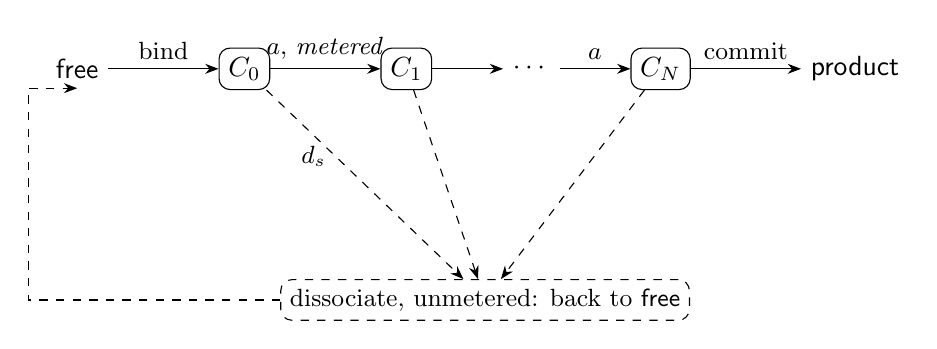
\begin{tikzpicture}[>=Stealth, node distance=15mm]
\node (free) {$\mathsf{free}$};
\node[draw, rounded corners, right=14mm of free] (c0) {$C_0$};
\node[draw, rounded corners, right=14mm of c0] (c1) {$C_1$};
\node[right=9mm of c1] (dots) {$\cdots$};
\node[draw, rounded corners, right=9mm of dots] (cn) {$C_N$};
\node[right=14mm of cn] (prod) {$\mathsf{product}$};
\draw[->] (free) -- node[above,font=\small] {bind} (c0);
\draw[->] (c0) -- node[above,font=\small] {$a$, \textit{metered}} (c1);
\draw[->] (c1) -- (dots);
\draw[->] (dots) -- node[above,font=\small] {$a$} (cn);
\draw[->] (cn) -- node[above,font=\small] {commit} (prod);
\node[draw, rounded corners, dashed, below=24mm of c1, xshift=10mm] (sink)
  {\small dissociate, unmetered: back to $\mathsf{free}$};
\foreach \n/\lab in {c0/$d_s$, c1/{}, cn/{}}{
  \draw[->,dashed] (\n) -- node[left,font=\small,pos=0.35] {\lab} (sink);
}
\draw[->,dashed] (sink.west) -- ++(-3.2,0) |- (free.south);
\end{tikzpicture}
\caption{One proofreading ladder. Solid arrows are funded base rules, one
token each. Dashed arrows are free: nothing is minted, and the candidate
simply ceases to exist as a candidate. The discrimination lives in the race at
each rung between a rate that does not depend on the substrate and one that
does.}
\label{fig:ladder}
\end{figure}

\section{Mapping into the graded \texttt{where}-clause framework}
\label{sec:mapping}

\subsection{What the framework already supplies}

The weighted graph-structured lambda theories of the companion note equip
rewrite rules with weight maps whose keys are spatial-behavioural formulae
refining the rule's left-hand side and whose values are weights in a
commutative semiring. Two rule classes are distinguished there, and the
distinction is exactly the one \S2 needs.

\begin{itemize}[leftmargin=*]
\item A \textbf{base rule} $\mathsf{r} \vdash (L) \leadsto (R)$ rewrites its
  redex. The redex is consumed. In the cost-accounted setting the firing must
  clear the funding judgement $\mathsf{funds}\;\Sigma\;\Delta := \Delta \leq
  \Sigma$; an unfunded rule has propensity zero.
\item A \textbf{context rule} $\mathsf{r} \mid S \leadsto T \vdash
  (\mathcal{C}\,S) \leadsto (\mathcal{C}\,T)$ contributes a multiplicative
  geometric factor $g(k)$ to the propensity of the rule it wraps, rather than
  an independent propensity of its own. Its left-hand side is restored. The
  energetics convention of the implementation states the position plainly:
  structural rules are addressing rather than dynamics, and incur no primitive
  cost.
\end{itemize}

\begin{observation}
A catalyst is a context rule and a pump is a base rule. This is not an
analogy that has to be argued for; it is what the two rule forms say.
\end{observation}

\subsection{The recognition test as a graded clause}

A recogniser is a for-comprehension carrying a graded \texttt{where}-clause.
The clause is a map from candidate matches into the resolution semiring $V$;
over $V = \Rnn$ its values are propensities, and the scheduler resolves the
race between enabled redexes in proportion to them.

One rung of a ladder is therefore \emph{two receives on one channel}, whose
relative weights are supplied by the clause: an advance arm and a dissociation
arm. Writing $\Kctx{\mathrm{adv}}$ and $\Kctx{\mathrm{off}}$ for the two
context-labelled modalities,
\[
\mathrm{Rung}_V(\psi) \;:=\;
\Kctx{\mathrm{adv}}_V \psi \;\oplus\; \Kctx{\mathrm{off}}_V \bot ,
\]
and a ladder of $N$ rungs is the $N$-fold nesting, which is the
budget-truncated unfolding of the least fixed point
\[
\mu X.\,\bigl(\grade{\beta} \oplus \Kctx{\mathrm{adv}}_V X\bigr) ,
\]
the width-engine schema of the choice-formulae note with the budget stopped at
$N$. The depth of the ladder is a budget on a fixed point, and that is the
first place the cost accounting enters: an unbounded $\mu$ is an unbounded
bill.

\subsection{Notation for the rest of the note}

Scale rates so that the right substrate dissociates at rate $1$ and the wrong
one at rate $f > 1$, with a common metered advance rate $a$. Per rung:
\[
p_r = \frac{a}{a+1}, \qquad
p_w = \frac{a}{a+f}, \qquad
g \;=\; \frac{p_r}{p_w} \;=\; \frac{a+f}{a+1} \;\leq\; f .
\]
$g$ is the discrimination one funded rung buys, $p_r$ the yield it costs.

\subsection{The Michaelis--Menten bound, as a proposition about rule classes}

\begin{proposition}[Michaelis--Menten bound]
\label{prop:mmbound}
Let a recogniser's recognition path be presented entirely by equations and
context rules --- no metered base rule between binding and commitment. Then
its discrimination is at most $f$, independently of the number of intermediate
states.
\end{proposition}

\begin{proof}[Argument]
Equations are symmetric and cost-free, and a context rule restores its
left-hand side and contributes a multiplicative factor to the propensity of
the rule it wraps rather than consuming anything. The internal chain therefore
satisfies detailed balance, and the steady-state occupancy ratio of the two
species depends only on the binding weights, not on the length of the chain.
Multiplying every forward and backward rate on a rung by the same factor
leaves the ratio fixed. Only a step that removes the intermediate from the
chain without a compensating reverse can make a rung a fresh test.
\end{proof}

\begin{proposition}[Funded advance multiplies]
\label{prop:multiplies}
If the advance is a base rule that consumes the intermediate, and a dissociated
candidate returns to the start rather than to the previous rung, then the
discrimination of an $N$-rung ladder is $g^{N}$.
\end{proposition}

Proposition~\ref{prop:mmbound} is verified numerically in \S\ref{sec:l1} by
solving both presentations on the same chain, and the two columns of
Table~\ref{tab:e1} are the whole argument of this note in numerical form.

\begin{principle}[Dissipation is the difference]
Selectivity beyond the equilibrium factor is bought, not engineered. In this
framework the purchase is visible in the syntax: it is the choice of rule
class, and the funding judgement is where the bill is presented.
\end{principle}

\section{Energy is the cost-accounting token}

\subsection{The ledger}

The mortal scientist's world conserves tokens: $\sigma + \kappa = \Theta$,
with $\sigma$ the purse, $\kappa$ the spend, $\Theta$ fixed, and nothing ever
minted. Every metered rewrite debits the purse, and a rule whose debit exceeds
the purse does not fire --- it is not slowed down, it has propensity zero.

This is the currency in which the price of accuracy is now denominated. There
is no need to import a thermodynamics: the ladder is spending the same tokens
the forager spends on food and the reproducing scientist spends on offspring,
and the three can therefore be compared.

\subsection{The exchange rate}

Charge one token per advance. Tokens are charged for candidates that are later
discarded, and for wrong candidates as well as right ones, since both are
entering. Then per candidate entering, the expected number of advances is
$p(1-p^{N})/(1-p)$, and the yield of accepted right candidates is $p_r^{N}$,
so the tokens per accepted right product are
\[
T(N) \;=\; \frac{1}{p_r^{N}}
\left[\frac{p_r(1-p_r^{N})}{1-p_r} + \frac{p_w(1-p_w^{N})}{1-p_w}\right] ,
\qquad
\varepsilon(N) = g^{-N},
\qquad
Y(N) = p_r^{N} .
\]

\begin{proposition}[The exchange rate is a power law]
\label{prop:power}
As $N$ grows, $\ln T(N) \sim N\ln(1/p_r)$ while $\ln(1/\varepsilon(N)) =
N \ln g$. Hence
\[
\varepsilon \;\sim\; T^{-\eta},
\qquad
\eta \;=\; \frac{\ln g}{\ln (1/p_r)} .
\]
Error falls as a \emph{power} of the tokens burned per accepted product.
\end{proposition}

\begin{remark}
This corrects a natural first guess. Counted per \emph{attempt}, accuracy does
look exponentially cheap, because the spend per attempt is bounded --- most
candidates are discarded early and never cost much. But a learner does not
eat attempts, it eats accepted products, and per acceptance the yield loss
compounds against it. \emph{The whole trade lives in yield}, and any account
that prices attempts rather than acceptances will overstate what dissipation
buys.
\end{remark}

\begin{proposition}[The rate does not depend on the depth]
\label{prop:depthfree}
$\eta$ is a function of $a$ and $f$ alone. Ladder depth converts tokens into
accuracy at this rate; it does not change the rate.
\end{proposition}

\subsection{What is scale-invariant is the rate}
\label{sec:scale}

Kinetic proofreading is usually reported to be scale-invariant by exhibition:
the same motif appears in cascade networks, in receptor discrimination, in
neural coincidence detection, in courtship, and in the promotion procedures of
organisations. Proposition~\ref{prop:depthfree} suggests a better statement.

The calculus builds terms with exactly two composition operators, prefixing
and parallel composition. Both the discrimination exponent and the token
spend are additive under both, under the appropriate independence conditions.
Their \emph{ratio} is therefore invariant under composition.

\begin{principle}[The price of accuracy is what recurs]
What is scale-invariant about kinetic proofreading is not the mechanism but
the exchange rate. The motif appears wherever computations compose because
composition is exactly what the rate is indifferent to.
\end{principle}

The two independence conditions are different, and the framework can state
both. \emph{Serial} independence is freshness: the advance must leave no
correlated residue in the new intermediate, which is the reset condition (c)
of \S2.2 and which the companion notes already discuss as freshness by
quotation. \emph{Parallel} independence is graded separation
$\varphi_i \mid_0^{\mathsf{N}} \varphi_j$, the factorisation theorem of the
composition note. Where either fails, the shortfall is measurable, and
\S\ref{sec:l3} measures it.

\begin{proposition}[Only composition multiplies]
\label{prop:onlycomp}
A single rung's discrimination is bounded by $f$ however much is spent on it:
$g(a) = (a+f)/(a+1) < f$ for all $a > 0$, with the bound approached only as
$a \to 0$, i.e.\ as the yield goes to zero.
\end{proposition}

This is why ladders exist at all, at every scale. A recogniser that wants
better than $f$ has no option but to compose, and composition is the only
operation available that multiplies.

\subsection{An optimum, and a negative result}
\label{sec:negative}

Because tokens are charged for discards, and discards grow with depth, there
is an interior optimum in the pair $(a, N)$ for any accuracy target. This is
already a contribution of token accounting: a rate-only account has no
principled stopping point, and a token account does.

The honest report, however, is that the optimum found here is a \emph{long}
ladder --- five to ten rungs for targets between $10^{-2}$ and $10^{-4}$ ---
whereas real proofreading ladders are one or two rungs. A per-rung holding
charge was tested, on the reasoning that an intermediate occupying a rung is
structure that must be kept and that keeping structure is metered. It does not
close the gap: raising the holding charge raises the cost without shortening
the ladder, because the higher yield available at a faster advance dominates.
Whatever makes biological ladders short is not this term. \S\ref{sec:l1}
records the numbers, and this is listed as an open problem rather than
resolved.

\section{What this adds to the learner's toolbox}
\label{sec:toolbox}

\subsection{Commitment, which the toolbox was missing}

The learner has a proposal mechanism (revision moves in the relaxation
lattice, with an ultrametric geometry and no gradient) and an evaluation
mechanism (the assay, with its trichotomy of confirm, refute, and bottom). It
has had almost nothing on \emph{commitment}.

That gap is exactly the seam the choice-formulae note names: a graded clause
is a quantifier, a map $\mathrm{Cand} \to V$, whereas a scheduler is a
selection function, a map into $\mathrm{Cand}$. The note says that the lift
from the first to the second is where the oracle lives, and prices the
altitude of the lift, but says nothing about its \emph{reliability}.

A proofreading ladder is that price. It sits precisely between weighing and
acting, it is made of the same clause language, and it converts a bounded
discrimination into an arbitrary one at a stated rate.

\begin{observation}
The swarm already exhibits the resulting division of labour: dance evaluation
is the clause, piping and takeoff are the selection, no bee does both, and
quorum sensing is the ladder in between~\cite{Seeley2010}. What was described
in the quorum note as a cost argument for sensing at the site rather than at
the cluster is a proofreading argument: the irreversible commitment is paid
for at interaction price.
\end{observation}

So the assay is not replaced. It becomes rung one of something that has a
depth dial, and the dial has a price.

\subsection{Energy substitutes for memory}

This is the part that seems to reach furthest.

Wald's sequential probability ratio test~\cite{Wald1945} achieves error
$\varepsilon$ in about $\ln(1/\varepsilon)/\ln g$ samples by accumulating a
log-likelihood ratio. It needs a register, and because it has one, an unlucky
early sample is recoverable: the accumulator simply moves back.

A proofreading ladder achieves the same scaling with \emph{no accumulator at
all}. The evidence is held in position on the ladder, write-once. Nothing is
summed, nothing is stored, and an unlucky sample is fatal --- the candidate is
gone.

\begin{principle}[The ratchet and the register]
Kinetic proofreading is the sequential likelihood-ratio test with the
accumulator replaced by a ratchet. The correct candidates it discards are the
register it declined to buy.
\end{principle}

This is a statement the framework can make quantitative, because holding
structure is already priced: the depth-graded schedule charges for the
formulae a learner keeps. Let $m$ be the price per step of holding the
accumulator, so a sequential test costs $\ln(1/\varepsilon)/\ln g \cdot (1+m)$
while the ladder costs $T(N)$. Equating gives a crossover memory price, and
\S\ref{sec:l2} computes it.

The reading is that \textbf{a learner too poor in memory to store its evidence
can buy the same discrimination by dissipating instead} --- and, in the
regime where memory is expensive, should. That is a genuine addition to the
toolbox: an instrument that trades one of the learner's scarce resources for
another, in a framework where both are denominated in the same tokens.

\subsection{Energy buys confidence, never scope}

Now the limitative result, and it is the one to state loudly.

The hypothesis space of the omnibus is a fibration: an ultrametric base of
formulae, and a $V$-valued fibre over each. A revision move changes the
formula, and so moves in the base. A proofreading rung changes the value
assigned to a candidate, and so moves \emph{only in the fibre}. A fibre move
has base-distance zero.

\begin{proposition}[Confinement is not relieved by dissipation]
\label{prop:confinement}
A proofreading ladder is a fibre operation. Consequently no amount of token
expenditure on proofreading moves a learner out of the ball it started in, and
the Confinement proposition applies to a well-funded learner exactly as it
applies to a poor one.
\end{proposition}

\begin{principle}[Energy buys confidence, never scope]
A well-funded science becomes maximally certain of the wrong ontology, and the
certainty is correctly earned. Nothing has gone wrong; the tokens really did
buy discrimination. They bought it inside a fibre.
\end{principle}

This has the same shape as the topen-boundary result of the quorum note --- a
shape error is unreachable by refinement --- and it is a contribution to the
question of why scientists get misled rather than to the ecology proper. It
also predicts an asymmetry worth looking for: richer scientific communities
should show \emph{sharper} disagreement across paradigm boundaries rather than
convergence, because each side is spending its surplus on confidence within
its own fibre.

\subsection{Two walls, one on each side}

Proofreading amplifies a discrimination the learner must already have. At
$f = 1$ no amount of energy helps: $g = 1$ for every $a$, and the ladder
returns exactly what it was given. That is the same statement as the forager's
bootstrap trap, where a value of zero is absorbing and a continuously enabled
receipt never fires.

So the toolbox now has a clean division of labour, with a wall at each end:

\begin{center}
\begin{tabular}{@{}lll@{}}
\toprule
 & \textbf{Exploration} & \textbf{Proofreading} \\
\midrule
Does what & manufactures a discrimination & amplifies one that exists \\
Efficiency & cannot be efficient & power law in tokens \\
Moves in & the base & the fibre \\
Wall & the bootstrap trap ($f = 1$) & the Michaelis--Menten bound \\
\bottomrule
\end{tabular}
\end{center}

Neither substitutes for the other, and a learner needs both. What
proofreading does \emph{not} add is anything at all about direction or
distance in the lattice. Most of learning is search rather than
discrimination, and this instrument is entirely on the discrimination side.

\section{Three levels of learning}

\subsection{Level 1: one recognition event}
\label{sec:l1}

\paragraph{Catalysis against dissipation.}
Both presentations are solved on the same $(N{+}1)$-state chain: the catalytic
presentation with reversible internal steps and dissociation only from $C_0$,
the proofread presentation with irreversible advance and dissociation from
every rung. Table~\ref{tab:e1} is Proposition~\ref{prop:mmbound} and
Proposition~\ref{prop:multiplies} side by side.

\begin{table}[h]
\centering
\begin{tabular}{@{}rrr@{}}
\toprule
$N$ & catalytic (restored) & proofread (consumed) \\
\midrule
0 & 0.10000900 & 0.10000900 \\
1 & 0.10000899 & 0.01089207 \\
2 & 0.10000898 & 0.00118626 \\
3 & 0.10000897 & 0.00012920 \\
4 & 0.10000896 & 0.00001407 \\
\bottomrule
\end{tabular}
\caption{Discrimination achieved, $f = 10$, $a = 0.1$. The catalytic column
is flat at $1/f$: adding steps to a presentation that restores its
intermediates buys nothing whatever. The residual $9\times10^{-6}$ is the
finite product drain used to make the steady state well posed.}
\label{tab:e1}
\end{table}

\paragraph{The exchange rate.}
Table~\ref{tab:e2} gives error, yield and tokens per accepted product for
$f = 10$, $a = 0.1$, where $g = 9.1818$ and $p_r = 0.0909$. The predicted
exponent is $\eta = \ln g / \ln (1/p_r) = 0.924655$; the measured local slope
between $N = 7$ and $N = 8$ is $0.924655$.

\begin{table}[h]
\centering
\begin{tabular}{@{}rrrrr@{}}
\toprule
$N$ & error & yield & tokens/acceptance & $\ln(1/\varepsilon)/\ln T$ \\
\midrule
1 & $1.089\times10^{-1}$ & 0.090909 & $1.109\times10^{0}$ & 21.4477 \\
2 & $1.186\times10^{-2}$ & 0.008264 & $1.321\times10^{1}$ & 1.7181 \\
3 & $1.292\times10^{-3}$ & 0.000751 & $1.463\times10^{2}$ & 1.3341 \\
4 & $1.407\times10^{-4}$ & 0.000068 & $1.610\times10^{3}$ & 1.2011 \\
5 & $1.532\times10^{-5}$ & 0.000006 & $1.772\times10^{4}$ & 1.1333 \\
6 & $1.669\times10^{-6}$ & 0.000001 & $1.949\times10^{5}$ & 1.0922 \\
7 & $1.818\times10^{-7}$ & --- & $2.144\times10^{6}$ & 1.0647 \\
8 & $1.980\times10^{-8}$ & --- & $2.358\times10^{7}$ & 1.0449 \\
\bottomrule
\end{tabular}
\caption{The exchange rate. Error falls as a power of tokens burned per
accepted product; the last column converges to $\eta$ from above.}
\label{tab:e2}
\end{table}

\paragraph{The rate belongs to one rung.}
Varying $a$ at fixed $f = 10$: $\eta = 0.5811$ at $a = 0.02$, $0.7419$ at
$0.05$, $0.9247$ at $0.1$, $1.4115$ at $0.3$, $2.4594$ at $1.0$, $4.0971$ at
$3.0$. Per factor of accuracy, many weak rungs are cheaper than a few strong
ones. Note that this is a statement about $a$ only; $N$ does not appear.

\paragraph{The optimum, and the negative result.}
Minimising tokens per acceptance over $(a, N)$ for a target error, with a
per-rung holding charge $c$:

\begin{center}
\begin{tabular}{@{}rrrrrr@{}}
\toprule
$c$ & target & best $a$ & best $N$ & tokens/acceptance & yield \\
\midrule
0 & $10^{-2}$ & 1.336 & 3 & 6.52 & 0.1870 \\
0 & $10^{-3}$ & 1.803 & 5 & 16.21 & 0.1101 \\
0 & $10^{-4}$ & 4.437 & 10 & 32.82 & 0.1310 \\
1 & $10^{-2}$ & 4.437 & 5 & 22.61 & 0.3619 \\
1 & $10^{-3}$ & 5.989 & 9 & 47.93 & 0.2492 \\
1 & $10^{-4}$ & 4.437 & 10 & 79.91 & 0.1310 \\
4 & $10^{-4}$ & 4.437 & 10 & 221.19 & 0.1310 \\
\bottomrule
\end{tabular}
\end{center}

The optimum is interior in both parameters even at $c = 0$, which is the
positive finding. The ladder it prefers is long, and the holding charge does
not shorten it. Recorded as open problem~\ref{op:short}.

\paragraph{Cross-check.}
Direct Monte Carlo at $f = 10$, $a = 1$, $N = 3$, four hundred thousand trials
per species, seed $20260817$: simulated error $0.006005$ against closed form
$0.006011$; yield $0.125305$ against $0.125000$; tokens per acceptance
$7.7931$ against $7.7994$.

\subsection{Level 2: one scientist}
\label{sec:l2}

\paragraph{The bottom rate is a bypass.}
A Hopfield ladder is destroyed by a bypass --- a path to commitment that skips
the rungs. Discrimination then saturates at the bypass fraction, however long
the ladder.

A mortal scientist has one, and it is already named in the corpus. The assay
that returns bottom because the \emph{observer} is underfunded is
indistinguishable from the assay that returns bottom because the
\emph{participant} is stuck. A scientist that must act anyway is taking the
bypass. Writing $b$ for the fraction of candidates that commit on bottom, the
error is
\[
\varepsilon_b(N) \;=\; b\,g^{-1} + (1-b)\,g^{-N},
\]
with floor $b/g$.

\begin{table}[h]
\centering
\begin{tabular}{@{}rrrrr@{}}
\toprule
$b$ & floor & $N^{*}$ (within 10\% of floor) & tokens at $N^{*}$ \\
\midrule
0 & --- & --- & --- \\
0.01 & $1.089\times10^{-3}$ & 5 & $1.772\times10^{4}$ \\
0.05 & $5.446\times10^{-3}$ & 4 & $1.610\times10^{3}$ \\
0.20 & $2.178\times10^{-2}$ & 3 & $1.463\times10^{2}$ \\
0.6104 & $6.648\times10^{-2}$ & 2 & $1.321\times10^{1}$ \\
\bottomrule
\end{tabular}
\caption{Past $N^{*}$ the tokens keep being spent and the accuracy does not
move. The two anchors $b = 0.6104$ at purse 60 and $b = 0$ at purse
$\geq 200$ are measured elsewhere in the corpus; intermediate values are
swept, not measured.}
\label{tab:e4}
\end{table}

\begin{principle}[Michaelis--Menten at both ends of the ladder]
With a bypass present, accuracy per token falls to zero at finite depth: the
exchange rate \emph{saturates in energy} the way the Michaelis--Menten rate law
saturates in substrate, and the bottom rate is playing the role of $K_M$.
\end{principle}

\begin{corollary}[Poverty caps accuracy, with a rate attached]
Since $b$ is a decreasing function of the purse, the maximum discrimination
available to a learner is bounded by its wealth, independently of how many
tokens it is willing to spend on the ladder. A poor learner cannot buy its way
to accuracy even if it spends everything, because what it is short of is the
ability to tell a refutation from an underfunded observation.
\end{corollary}

\begin{figure}[t]
\centering
\begin{tikzpicture}[x=0.72cm,y=0.66cm,>=Stealth]
\draw[->] (-0.3,0) -- (8.2,0) node[right,font=\small] {$\log_{10} T$};
\draw[->] (0,-0.3) -- (0,8.4) node[above,font=\small] {$\log_{10}(1/\varepsilon)$};
\foreach \x in {0,2,4,6} \draw (\x,0.08) -- (\x,-0.08) node[below,font=\scriptsize] {\x};
\foreach \y in {0,2,4,6,8} \draw (0.08,\y) -- (-0.08,\y) node[left,font=\scriptsize] {\y};
\draw[thick] (0.045,0.963) -- (1.121,1.926) -- (2.165,2.889) -- (3.207,3.852)
             -- (4.249,4.815) -- (5.290,5.778) -- (6.331,6.741) -- (7.373,7.703);
\node[right,font=\small] at (7.0,7.4) {$b=0$};
\draw[thick,dashed] (0.045,0.963) -- (1.121,1.777) -- (2.165,2.176)
             -- (3.207,2.253) -- (4.249,2.263) -- (5.290,2.264)
             -- (6.331,2.264) -- (7.373,2.264);
\node[right,font=\small] at (6.4,1.85) {$b=0.05$};
\draw[dotted] (0,2.264) -- (7.6,2.264);
\node[left,font=\scriptsize] at (0,2.264) {};
\end{tikzpicture}
\caption{The exchange rate, with and without a bypass. Without one, accuracy
is a straight line in tokens on log--log axes, of slope $\eta = 0.9247$. With
a bypass at five per cent, the curve saturates: past four rungs the tokens buy
nothing. The ceiling is set by $b$ and cannot be raised by spending.}
\label{fig:rate}
\end{figure}

\paragraph{The ratchet against the register.}
Giving the sequential test exactly the evidence one rung extracts, so that the
comparison is between bookkeeping schemes rather than between tests:

\begin{center}
\begin{tabular}{@{}rrrrr@{}}
\toprule
target & ladder $N$ & ladder tokens & sequential samples & crossover price $m$ \\
\midrule
$10^{-2}$ & 3 & $1.463\times10^{2}$ & 2.077 & 69.4 \\
$10^{-3}$ & 4 & $1.610\times10^{3}$ & 3.115 & 515.9 \\
$10^{-4}$ & 5 & $1.772\times10^{4}$ & 4.154 & 4263.7 \\
$10^{-6}$ & 7 & $2.144\times10^{6}$ & 6.231 & 344019.5 \\
\bottomrule
\end{tabular}
\end{center}

The crossover price is where the ratchet becomes the cheaper instrument, and
it climbs steeply with the accuracy demanded. The fraction of \emph{correct}
candidates discarded at these settings is $0.999249$, $0.999932$, $0.999994$
and $1.000000$ respectively --- and that column is the honest statement of
what the ladder paid.

\begin{observation}
At this advance rate the register is enormously the better buy unless memory
is hundreds of times more expensive than a rewrite. That is a substantive
prediction, not a disappointment: it says that a learner with any usable
memory at all should accumulate rather than ratchet, and that ratcheting is
the instrument of learners whose state cannot be held --- which is exactly the
situation of a molecular recogniser, and exactly the situation of a
population whose members cannot share a register.
\end{observation}

\subsection{Level 3: a population}
\label{sec:l3}

A population is a converter too. Each reviewer is a rung; rejection is the
discard arm; the tokens are the reviewers' own. The question the framework can
now ask sharply is whether the exchange rate survives aggregation.

Reviewers are modelled as weak tests calibrated to the same $(p_r, p_w)$, with
a shared latent component of weight $k$ and a private component of weight
$1-k$: $k = 0$ is disjoint namespaces, $k = 1$ is one reviewer wearing $m$
hats. The effective exponent is $n_{\mathrm{eff}} = \ln(1/\varepsilon)/\ln g$,
and $n_{\mathrm{eff}}/m$ is the fraction of burned tokens that became
discrimination.

\begin{table}[h]
\centering
\begin{tabular}{@{}rrrrr@{}}
\toprule
$k$ & $m=1$ & $m=2$ & $m=4$ & $m=8$ \\
\midrule
0.00 & 0.9969 & 0.9949 & 1.0028 & 1.0026 \\
0.25 & 1.0039 & 0.8962 & 0.7545 & 0.5825 \\
0.50 & 0.9961 & 0.7948 & 0.5862 & 0.4022 \\
0.75 & 1.0066 & 0.6958 & 0.4471 & 0.2788 \\
1.00 & 0.9948 & 0.4992 & 0.2490 & 0.1246 \\
\bottomrule
\end{tabular}
\caption{$n_{\mathrm{eff}}/m$, the efficiency of the population as a converter.
Two hundred thousand trials per cell, seed $20260818$, reviewers calibrated to
$g = 1.5$. At $k = 0$ the reviewers multiply and every token converts. At
$k = 1$ the column is $1/m$ to three figures: the other $m-1$ reviewers bought
nothing at all.}
\label{tab:e6}
\end{table}

\begin{principle}[Overlap is a tax on the exchange rate]
Correlation between stages is not a combinatorial nuisance but a
thermodynamic inefficiency, and $n_{\mathrm{eff}}/m$ measures it. A population
of correlated reviewers is a lossy converter, and the loss is computable from
the grading vector.
\end{principle}

\begin{observation}[A replication crisis is an efficiency collapse]
The observable signature is specific: adding reviewers continues to cost and
stops discriminating. It is not that the reviewers are bad --- each row of
Table~\ref{tab:e6} has the same $m=1$ entry --- but that they are not
independent stages. The remedy the framework suggests is not more review but
disjoint namespaces, and the grading vector says what that means.
\end{observation}

Finally, Proposition~\ref{prop:onlycomp} in numbers. Against $m$ disjoint rungs
giving $1.089\times10^{-1}$, $1.186\times10^{-2}$, $1.292\times10^{-3}$,
$1.407\times10^{-4}$, $1.669\times10^{-6}$, $1.980\times10^{-8}$ for
$m = 1,2,3,4,6,8$, a single rung with the advance slowed $m$-fold gives
$1.089\times10^{-1}$, $1.045\times10^{-1}$, $1.030\times10^{-1}$,
$1.022\times10^{-1}$, $1.015\times10^{-1}$, $1.011\times10^{-1}$ --- creeping
towards $1/f = 0.1$ and never past it. Spending more on one rung does not
multiply. Only composition multiplies.

\section{The ladder in rholang}
\label{sec:code}

The listing below is written in the conventions of the companion notes:
\texttt{new} is sugar, intermediates are manufactured by quotation, and a
parameter written \texttt{c} is a name while \texttt{@d} is data.

\begin{lstlisting}
// ---------------------------------------------------------------
// One rung.  The two arms are TWO RECEIVES ON ONE CHANNEL, so the
// scheduler resolves a race between them, and the graded where-clause
// supplies the weights.  Only the advance arm is metered.
// ---------------------------------------------------------------
contract rung(@k, cand, up, waste, budget) = {
    // advance: a funded base rule.  The gate {% P %}[s] fires only if
    // the budget stack can cover the debit; unfunded means propensity
    // zero, not a slower rate.
    for (@c <- cand where bindsAt(c, k)) {
      {% up!( quoteFresh(c, k) ) %}[ advance ]
    }
  |
    // dissociate: unmetered.  The intermediate is dropped, and the
    // candidate must start again from the bottom.  Nothing is minted
    // and nothing is restored: this arm is where irreversibility lives.
    for (@c <- cand where bindsAt(c, k)) {
      waste!(c)
    }
}

// ---------------------------------------------------------------
// The ladder.  Rungs are composed in parallel over a chain of
// manufactured names, so the ladder is literally the N-fold
// composition of one rung.
// ---------------------------------------------------------------
contract ladder(@n, inp, out, waste, budget) = {
  match n {
    0  => for (@c <- inp) { out!(c) }
    _  => {
      // a name fresh in the current scope, by quotation
      new mid in {
        rung!(n, *inp, *mid, *waste, *budget)
      | ladder!(n - 1, *mid, *out, *waste, *budget)
      }
    }
  }
}

// ---------------------------------------------------------------
// The recogniser.  Perception must not be able to act: the arm that
// READS a candidate and the arm that ADVANCES it are on different
// namespaces, or looking at a candidate would promote it.
// ---------------------------------------------------------------
contract recognise(@n, source, verdict, budget) = {
  new inp, out, waste in {
    for (@c <= source) { inp!(c) }             // peek, not consume
  | ladder!(n, *inp, *out, *waste, *budget)
  | for (@c <- out) { verdict!("commit", c) }
  | for (@c <- waste) { Nil }                  // the discard is silent
  }
}
\end{lstlisting}

Two points about the listing are the substance rather than the syntax. First,
the gate \texttt{\{\% P \%\}[advance]} on the advance arm and its absence on
the dissociation arm is the entire Michaelis--Menten/proofreading distinction,
written down. Second, the separation of the reading namespace from the
advancing namespace is forced, and for the same reason it was forced in the
game note and the quorum note: an observer that can advance a candidate by
looking at it is not observing.

\section{What is shown, what is not, and what is open}

\subsection{Shown}

\begin{enumerate}[leftmargin=*,label=(\arabic*)]
\item The Michaelis--Menten bound holds as a statement about rule classes
  (Proposition~\ref{prop:mmbound}), and the two presentations differ
  numerically by four orders of magnitude at four rungs (Table~\ref{tab:e1}).
\item The exchange rate is a power law in tokens per acceptance with exponent
  $\eta = \ln g/\ln(1/p_r)$, verified to six figures
  (Proposition~\ref{prop:power}, Table~\ref{tab:e2}).
\item The exponent is a property of one rung, so ladder depth converts at a
  fixed rate rather than changing it (Proposition~\ref{prop:depthfree}).
\item Only composition multiplies discrimination
  (Proposition~\ref{prop:onlycomp}, \S\ref{sec:l3}).
\item A bypass caps discrimination, and the mortal scientist's bottom rate is
  a bypass; accuracy per token reaches zero at finite depth
  (Table~\ref{tab:e4}).
\item Correlated stages are a lossy converter, with $n_{\mathrm{eff}}/m = 1/m$
  at full overlap to three figures (Table~\ref{tab:e6}).
\item Token accounting supplies an interior optimum in $(a, N)$ where a
  rate-only account supplies none.
\end{enumerate}

\subsection{Not shown}

The claim that a proofreading rung is a fibre move
(Proposition~\ref{prop:confinement}) is argued informally from the fibration
reading of the omnibus, which is itself flagged there as assembled rather than
established. The ratchet/register comparison prices memory by stipulation; the
crossover figures are only as good as that stipulation, and the sensitivity
sweep in \S\ref{sec:l2} is offered in place of a justification. Nothing here
is a claim about biology: the models are the textbook idealisations, and the
one place where the idealisation is confronted with the biology --- ladder
length --- it loses.

\subsection{Open problems}

\begin{enumerate}[leftmargin=*,label=O\arabic*.]
\item\label{op:short} \textbf{Why are real ladders short?} The optimum computed
  here is five to ten rungs; biology uses one or two. The per-rung holding
  charge does not close the gap. Candidates: a fixed cost of installing a
  rung that is amortised over many recognitions rather than charged per
  candidate; a constraint from the assembly index of the apparatus; or a
  yield floor imposed by the ecology rather than by the recogniser.
\item \textbf{Is the conversion bound the thermodynamic uncertainty relation
  in a costume?} A bound of the shape $\ln(1/\varepsilon) \leq 1 + \kappa/
  \mathrm{price}$ should be provable from conservation plus the
  equation/rewrite split alone. Whether that is a new bound or a restatement
  of the results of Barato and Seifert~\cite{BS2015} and
  Lan et al.~\cite{Lan2012} needs a literature pass before any claim is made.
  The interesting possibility is not the bound but its provenance: a calculus
  built for concurrency having a second law because it distinguishes equations
  from rewrites.
\item \textbf{The quantum rung.} The unitary dilation of the companion note
  supplies an ancilla, and a discarded candidate is exactly what gets swept
  into it. Conjecture: the ancilla resource required is the tokens burned. If
  so, interference cannot buy discrimination for free, which would close the
  question the weighted-GSLT note left open.
\item \textbf{Learning the overlap.} $n_{\mathrm{eff}}/m$ is measurable by a
  population about itself. A population that could estimate its own
  efficiency could reallocate reviewers, which is a graded-clause problem of
  the kind the composition note poses but does not solve.
\item \textbf{Does the ratchet ever win in a mortal setting?} The crossover
  prices computed here are high. Populations whose members cannot share a
  register are the obvious candidate, and the swarm is the obvious test case.
\end{enumerate}

\begin{thebibliography}{99}

\bibitem{BS2015} A.~C. Barato and U. Seifert.
  Thermodynamic uncertainty relation for biomolecular processes.
  \emph{Physical Review Letters}, 114:158101, 2015.

\bibitem{Bennett1982} C.~H. Bennett.
  The thermodynamics of computation --- a review.
  \emph{International Journal of Theoretical Physics}, 21:905--940, 1982.

\bibitem{BH1925} G.~E. Briggs and J.~B.~S. Haldane.
  A note on the kinetics of enzyme action.
  \emph{Biochemical Journal}, 19:338--339, 1925.

\bibitem{Hopfield1974} J.~J. Hopfield.
  Kinetic proofreading: a new mechanism for reducing errors in biosynthetic
  processes requiring high specificity.
  \emph{Proceedings of the National Academy of Sciences}, 71:4135--4139, 1974.

\bibitem{Landauer1961} R. Landauer.
  Irreversibility and heat generation in the computing process.
  \emph{IBM Journal of Research and Development}, 5:183--191, 1961.

\bibitem{Lan2012} G. Lan, P. Sartori, S. Neumann, V. Sourjik and Y. Tu.
  The energy--speed--accuracy trade-off in sensory adaptation.
  \emph{Nature Physics}, 8:422--428, 2012.

\bibitem{McKeithan1995} T.~W. McKeithan.
  Kinetic proofreading in T-cell receptor signal transduction.
  \emph{Proceedings of the National Academy of Sciences}, 92:5042--5046, 1995.

\bibitem{MM1913} L. Michaelis and M.~L. Menten.
  Die Kinetik der Invertinwirkung.
  \emph{Biochemische Zeitschrift}, 49:333--369, 1913.

\bibitem{Murugan2012} A. Murugan, D.~A. Huse and S. Leibler.
  Speed, dissipation, and error in kinetic proofreading.
  \emph{Proceedings of the National Academy of Sciences}, 109:12034--12039,
  2012.

\bibitem{Ninio1975} J. Ninio.
  Kinetic amplification of enzyme discrimination.
  \emph{Biochimie}, 57:587--595, 1975.

\bibitem{Seeley2010} T.~D. Seeley.
  \emph{Honeybee Democracy}. Princeton University Press, 2010.

\bibitem{Wald1945} A. Wald.
  Sequential tests of statistical hypotheses.
  \emph{Annals of Mathematical Statistics}, 16:117--186, 1945.

\bibitem{Sci} L.~G. Meredith.
  The Mortal Scientist: learning as cost-accounted computation in a reflective
  higher-order calculus. F1R3FLY.io research note, 2026.

\bibitem{Game} L.~G. Meredith.
  Learning to Play. F1R3FLY.io research note, 2026.

\bibitem{Compose} L.~G. Meredith.
  Composing Learners. F1R3FLY.io research note, 2026.

\bibitem{Weighted} L.~G. Meredith.
  Weighted Graph-Structured Lambda Theories: stochastic and quantum execution
  for MeTTaIL. F1R3FLY.io research note, second version, 2026.

\bibitem{Graded} L.~G. Meredith.
  Graded Where-Clauses. F1R3FLY.io research note, 2026.

\bibitem{Choice} L.~G. Meredith.
  Choice Principles as Graded Where-Clauses. F1R3FLY.io research note, 2026.

\bibitem{Quorum} L.~G. Meredith.
  Quorum as a Where-Clause. F1R3FLY.io research note, 2026.

\bibitem{Omnibus} L.~G. Meredith.
  Observation Disciplines. F1R3FLY.io omnibus, 2026.

\end{thebibliography}

\end{document}
